\chapter{Experiments and Results}
\label{ch:experiments}

This chapter presents the results of experiments conducted on the three datasets using classification and clustering techniques. All experiments were performed in a Jupyter Notebook environment using Python.

%%%%%%%%%%%%%%%%%%%%%%%%%%%%%%%%%%%%%%%%%%
\section{D-1: Raisin Dataset (Classification)}
\label{sec:results_raisin}

\subsection{Model Training and Evaluation}

Both KNN and Naïve Bayes were tested using progressively increasing feature subsets. The dataset was first preprocessed, scaled, and label encoded.

\begin{lstlisting}[language=Python, caption={Training KNN with increasing features}, label=list:raisin_knn]
for i in range(2, len(features) + 1):
    selected = features[:i]
    X = df_raisin[selected]
    y = LabelEncoder().fit_transform(df_raisin['Class'])

    X_scaled = StandardScaler().fit_transform(X)
    X_train, X_test, y_train, y_test = train_test_split(X_scaled, y)

    acc, cm = train_knn(X_train, y_train, X_test, y_test, n_neighbors=3)
    print(f"{i} features -> Accuracy: {acc}")
\end{lstlisting}

\subsection{KNN vs Naïve Bayes Performance}

\begin{table}[H]
\centering
\caption{KNN vs Naïve Bayes Accuracy across Features (Raisin)}
\label{tab:raisin_accuracy}
\begin{tabular}{|c|c|c|}
\hline
\# Features & KNN Accuracy & Naïve Bayes Accuracy \\
\hline
2 & 80.00\% & 85.00\% \\
3 & 80.00\% & 82.22\% \\
4 & 80.00\% & 82.22\% \\
5 & 82.22\% & 82.78\% \\
6 & 82.22\% & 82.78\% \\
7 & 82.22\% & 82.78\% \\
\hline
\end{tabular}
\end{table}

\begin{figure}[H]
    \centering
    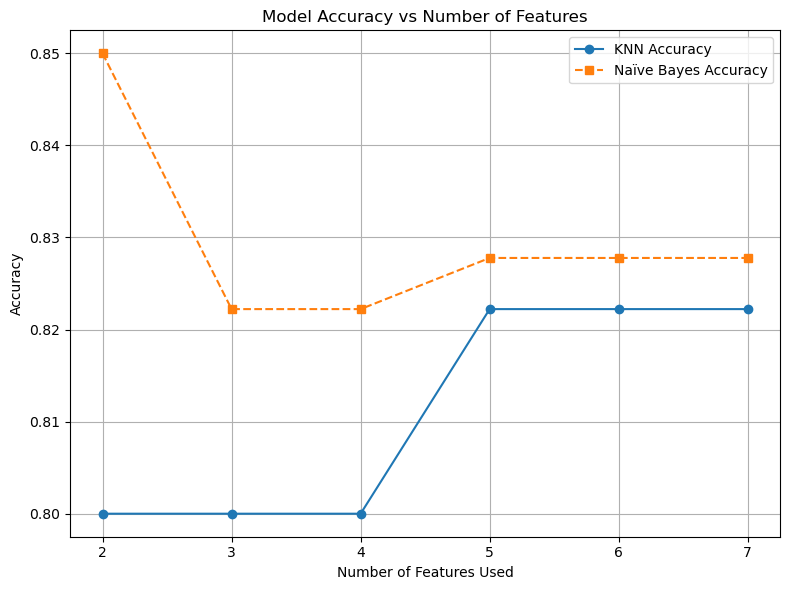
\includegraphics[width=0.6\textwidth]{figures/raisin_accuracy_plot.png}
    \caption{Accuracy comparison for KNN vs Naïve Bayes (Raisin)}
    \label{fig:raisin_accuracy}
\end{figure}

\subsection{Observations}
Naïve Bayes achieved its best performance using just two features (85\%), while KNN improved gradually with more features. Both models plateaued at ~82\% when all features were used.

%%%%%%%%%%%%%%%%%%%%%%%%%%%%%%%%%%%%%%%%%%
\section{D-2: HTRU2 Dataset (Classification)}
\label{sec:results_htru2}

\subsection{Model Execution}

HTRU2 presented a more complex dataset, where both classifiers were evaluated for accuracy using all features.

\begin{lstlisting}[language=Python, caption={Confusion matrix for KNN on HTRU2}, label=list:htru2_cm]
# KNN with all 8 features
X_scaled = StandardScaler().fit_transform(df_htru.drop('Class', axis=1))
y = df_htru['Class']
X_train, X_test, y_train, y_test = train_test_split(X_scaled, y)

acc, cm = train_knn(X_train, y_train, X_test, y_test, n_neighbors=5)
print(f"KNN Accuracy: {acc}")
print("Confusion Matrix:\n", cm)
\end{lstlisting}

\subsection{Best Performance Snapshot}

\begin{table}[H]
\centering
\caption{HTRU2 KNN Confusion Matrix (98.27\% Accuracy)}
\label{tab:htru2_confusion}
\begin{tabular}{|c|c|c|}
\hline
           & Predicted 0 & Predicted 1 \\
\hline
Actual 0   & 3242        & 17           \\
Actual 1   & 45          & 276          \\
\hline
\end{tabular}
\end{table}

\begin{figure}[H]
    \centering
    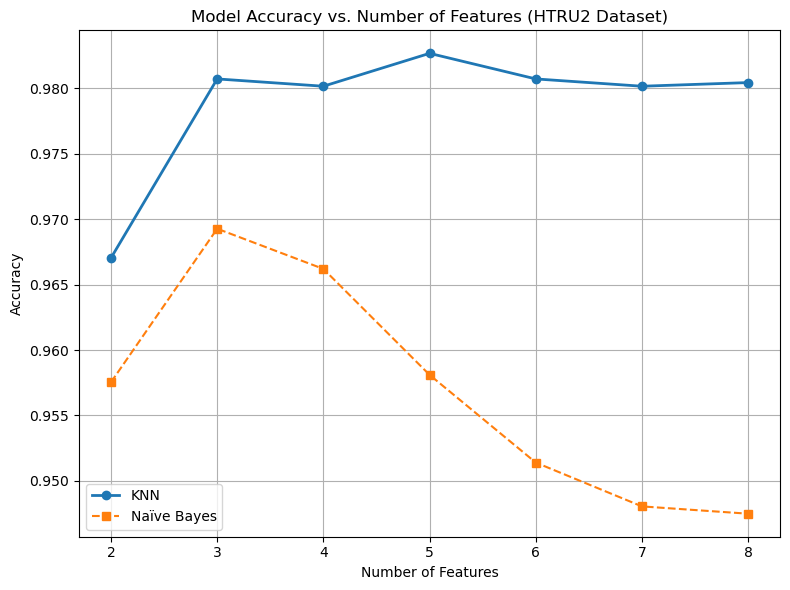
\includegraphics[width=0.6\textwidth]{figures/htru2_accuracy_plot.png}
    \caption{KNN vs Naïve Bayes on HTRU2 Dataset}
    \label{fig:htru2_accuracy}
\end{figure}

\subsection{Observations}

KNN achieved a remarkable 98.27\% accuracy on the HTRU2 dataset, outperforming Naïve Bayes significantly. This confirms KNN’s strength with high-dimensional, numeric data.

%%%%%%%%%%%%%%%%%%%%%%%%%%%%%%%%%%%%%%%%%%
\section{D-3: Parking Birmingham Dataset (Clustering)}
\label{sec:results_parking}

\subsection{K-Means Clustering}

\begin{lstlisting}[language=Python, caption={Elbow Method for Optimal K}, label=list:elbow]
inertia = []
for k in range(1, 11):
    kmeans = KMeans(n_clusters=k).fit(X_scaled)
    inertia.append(kmeans.inertia_)
\end{lstlisting}

\begin{figure}[H]
    \centering
    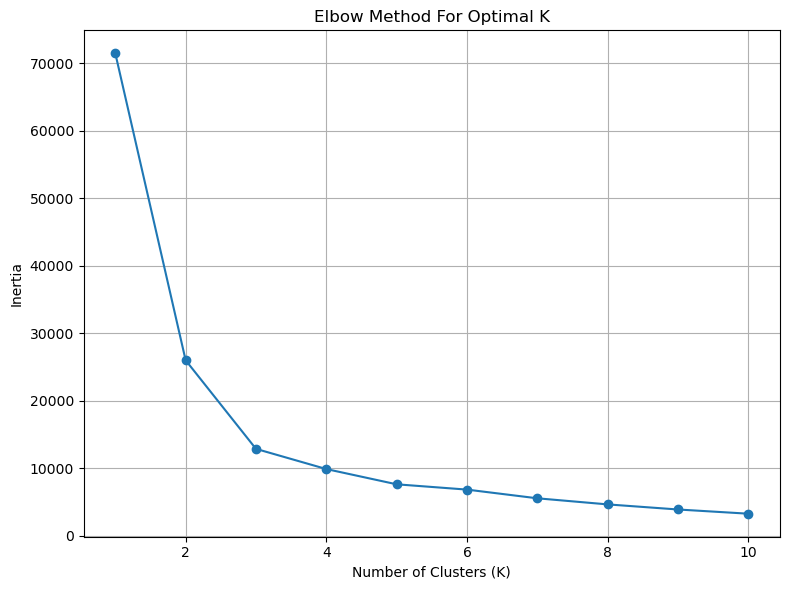
\includegraphics[width=0.6\textwidth]{figures/parking_elbow_plot.png}
    \caption{Elbow Method showing inflection at $K=3$}
    \label{fig:parking_elbow}
\end{figure}

\subsection{Clustering Visualization}

\begin{figure}[H]
    \centering
    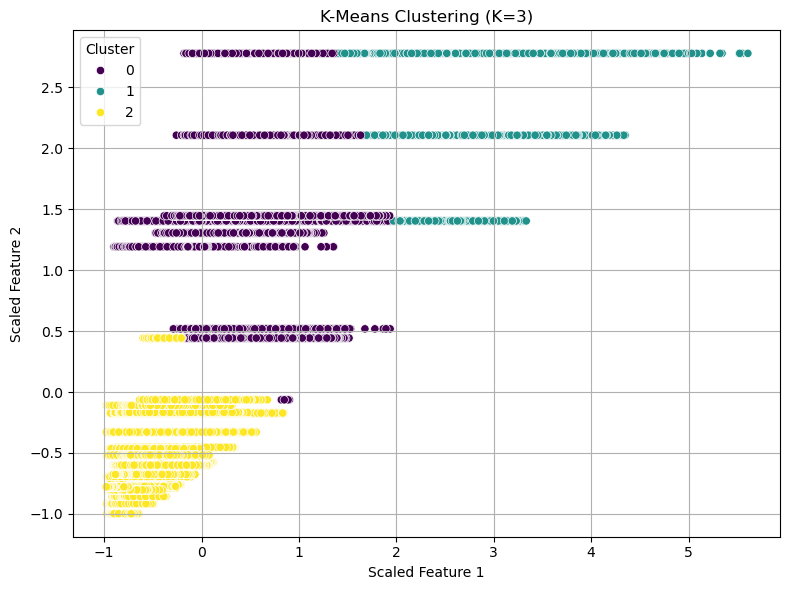
\includegraphics[width=0.6\textwidth]{figures/parking_clusters_k3.png}
    \caption{Parking Clusters for $K=3$}
    \label{fig:parking_clusters_k3}
\end{figure}

\subsection{Observations}

The Elbow Method suggested $K=3$ as optimal. Clusters revealed patterns of low, medium, and high occupancy. K=4 was also tested but led to overlapping and less interpretable groupings.

%%%%%%%%%%%%%%%%%%%%%%%%%%%%%%%%%%%%%%%%%%
\section{Summary}

This chapter demonstrated how machine learning models performed across datasets and under varying conditions. Results support the use of KNN in numeric classification problems and highlight the interpretability of K-Means when clusters are well separated.